\documentclass[conference]{IEEEtran}
\usepackage{array}
\usepackage{booktabs}
\usepackage{calc}
\usepackage{url}
\Urlmuskip=0mu\relax
\hyphenation{off-line}
\usepackage{textcomp}
\usepackage{fancyvrb}
\usepackage{graphicx}
\usepackage{tikz}
\usetikzlibrary{positioning,arrows.meta}
\newcommand{\real}[1]{#1}
\providecommand{\tightlist}{\setlength{\itemsep}{0pt}\setlength{\parskip}{0pt}}
\makeatletter
\def\verbatim@font{\ttfamily\scriptsize}
\makeatother
\begin{document}
\title{Seppa: Correctness-Gated LLM Kernel Optimization on the Raspberry Pi 5 GPU}
\author{\IEEEauthorblockN{Adam Munawar Rahman}
\IEEEauthorblockA{New York University \\ New York, NY, USA \\ msr541@nyu.edu \\ ECE-GY 9953 Advanced Project. Adviser: Prof.\ Brandon Reagen}}
\maketitle
\begin{abstract}
Most edge AI deployments on single-board computers leave the integrated
GPU idle. We present Seppa, a harness that puts a large language model
in the loop for optimizing GPU kernels, the small programs a GPU runs in
parallel: the model proposes changes, and a finite-state machine
compiles, verifies against physics-based correctness gates, benchmarks,
and decides keep or revert, refusing to benchmark any kernel that failed
verification. On the flood-simulation stencil (a kernel in which each
grid cell updates from its neighbors) of an offline flood-guidance
application for the Raspberry Pi 5, a hand-driven sweep through the same
gates produced a kernel 1.58x faster than the original. The machine
re-measured and re-judged the result in five consecutive runs driven
from a second computer, and in every run it refused to benchmark a
kernel that failed its gate. With CPU inference running concurrently the
advantage widens to 2.20x, and the deployment sustains 9.6 tokens/s of
language-model decode (token-by-token text generation) beside 883
simulation steps per second, an operating point that beats the best
measured CPU-only configuration on both axes in the steady-state
campaign.
\end{abstract}
\begin{IEEEkeywords}
GPU kernel optimization, LLM agents, correctness verification, edge computing, Vulkan
\end{IEEEkeywords}
\section{Introduction}\label{introduction}

Raspberry Pi class boards are a common platform for edge AI in
emergency-response and field settings, where power, connectivity, and
budget are constrained {[}12{]} and inference must happen on-device once
the network is gone {[}11{]}. A Pi 5 runs a quantized billion-parameter
model (weights compressed to low-precision integers) on its CPU cores
{[}8{]}, generating text one token, roughly a word fragment, at a time,
in the phase called decode. AI capability is usually added with
dedicated hardware, a neural-processing add-on board (NPU HAT) or a USB
accelerator {[}13{]}, which raises cost and adds a procurement
dependency in a supply-constrained chip market {[}14{]}.

Less attention goes to silicon already on the board: every Pi 5 ships a
VideoCore VII GPU (the V3D) that compute workloads rarely touch, and
during CPU inference it idles. Two questions decide that idle GPU's
worth: whether it can be made fast enough at a useful workload to be a
co-processor, and whether it can run beside a busy CPU on a shared LPDDR
bus. The case study (Section V) and its machine-checked reproduction
(Section VI) take up the first question; the concurrency measurements
(Section VII) take up the second.

The V3D is a mobile GPU with sparse documentation, and tuning habits
learned on NVIDIA hardware, the target of most optimization literature,
largely fail on it (Section II gives the background). Empirical, poorly
documented work of this kind is what the field has begun handing to
language models. The existing tools are agentic optimizers: loops that
put the model in charge of every step, including checking its own
results. AutoKernel {[}15{]} is one. These loops steer the model with
prompts and trust it to verify honestly and revert bad kernels, and
Section III's related work shows that trust has a poor record. Seppa
removes the trust by narrowing the model's role: the model proposes, and
nothing else. A finite-state machine built on Apache Burr {[}5{]}, a
Python state-machine library, owns compilation, verification,
benchmarking, and the verdict, and refuses out-of-order requests. The
machine is served over the Model Context Protocol (MCP) {[}6{]}, a
standard interface through which a language model calls tools on a
server.

The demonstration workload is the flood simulation of an offline
flood-guidance application {[}7{]}, which must run beside language-model
narration on one board. Its core kernel is a stencil, a computation that
updates every cell of a grid from its neighbors each step; that kernel
is the optimization target, and the application's CPU-plus-GPU split is
what we measure (Section IX describes the application).

One boundary should be drawn now. This paper shows that a machine can
verify, reproduce, and police the model's results. It does not show that
the model can find good optimizations on its own; that remains untested
here. Within that boundary, the paper reports:

\begin{enumerate}
\def\labelenumi{\arabic{enumi}.}
\tightlist
\item
  the optimization of a real flood stencil for the Pi's V3D GPU under
  three physics gates (correctness checks passed before any benchmark),
  to 1.58x, failed hypotheses included (Section V);
\item
  an action-space lesson: the first search plateaued because every
  winning change lived in the host program (the CPU-side code that
  allocates buffers and launches the kernel), outside what the machine
  let the model edit (Section V-C);
\item
  a machine-checked reproduction over MCP, repeated five times under a
  defined pass criterion, including the server's refusal to benchmark a
  gate-failing kernel (Section VI);
\item
  an interference measurement of the deployed configuration against a
  gate-verified CPU-only counterfactual (Section VII). In the
  steady-state campaign the GPU split beats the partitioned scheme, the
  strongest CPU-only arrangement, on both axes, and it never trails that
  scheme in any campaign measured.
\end{enumerate}

\section{Background: The Raspberry Pi 5
GPU}\label{background-the-raspberry-pi-5-gpu}

The Pi 5 pairs four Cortex-A76 CPU cores with a VideoCore VII GPU (V3D
7.1), the block that also drives the desktop. There is no CUDA and no
vendor compute toolchain; compute reaches the GPU only through Vulkan
shaders, small programs the GPU runs many times in parallel, compiled by
Mesa's v3dv driver {[}9{]}. In this paper, kernel means a GLSL compute
shader.

Tables~\ref{tab:platform} and \ref{tab:gpu} list the
platform and the GPU's compute limits, collected from the running board
by \texttt{pi/collect\_specs.sh} (archived with the raw vulkaninfo
dump). The limits are tight, and the scale is modest: the best kernel we
measured sustains about 13 GFLOP/s in fp32, and that figure belongs to a
dense matrix multiply (Section VII-A compares the processors on the
stencil itself). The GPU is a second, slower engine that happens to be
free. In Vulkan's terms, a dispatch is one launch of a kernel over the
whole grid; one invocation is one execution of the kernel by one GPU
thread; invocations are grouped into workgroups, and the hardware runs
them in lockstep bundles of 16 called subgroups.

{\def\LTcaptype{none} % do not increment counter
\begin{table}[!t]\caption{Platform, collected from the running board by \mbox{collect\_specs.sh}}\label{tab:platform}\centering\footnotesize\setlength{\tabcolsep}{2.5pt}\renewcommand{\arraystretch}{1.15}\begin{tabular}{@{}
  >{\raggedright\arraybackslash}p{(\linewidth - 2\tabcolsep) * \real{0.5000}}
  >{\raggedright\arraybackslash}p{(\linewidth - 2\tabcolsep) * \real{0.5000}}@{}}
\toprule
Model & Raspberry Pi 5 Model B Rev 1.1 \\
SoC & BCM2712 \\
CPU & 4 x Cortex-A76 @ 2400 MHz \\
RAM & 16 GB LPDDR (shared with GPU) \\
OS / kernel & Debian GNU/Linux 13 (trixie) (DietPi 10.5.2),
6.18.39+rpt-rpi-2712 \\
Firmware & 2025/12/08 \\
\bottomrule
\end{tabular}\end{table}
}

{\def\LTcaptype{none} % do not increment counter
\begin{table}[!t]\caption{GPU compute limits, collected live (vulkaninfo)}\label{tab:gpu}\centering\footnotesize\setlength{\tabcolsep}{2.5pt}\renewcommand{\arraystretch}{1.15}\begin{tabular}{@{}ll@{}}
\toprule
Device & V3D 7.1.10.2 \\
Driver & Mesa 25.0.7-2+rpt4 (v3dv) \\
Vulkan API & 1.3.305 \\
Core clock & 960 MHz \\
Max invocations / workgroup & 256 \\
Shared memory / workgroup & 16 KB \\
Subgroup (SIMD) width & 16 \\
fp16 arithmetic & no \\
Cooperative matrix & no \\
\bottomrule
\end{tabular}\end{table}
}

The strange part is the driver: when a shader wants more registers than
exist, v3dv does not fail. It walks a ladder of thirteen compile
strategies {[}16{]}, disabling the optimizations that spend registers
for speed (instruction scheduling, code motion, loop unrolling, load
sorting, pipelining) one at a time. It then halves the thread count,
repeats the disables, and ends on a fallback scheduler, handing back
whatever survives, sometimes several times slower.

\section{Related Work}\label{related-work}

Kernel generation is now a standard LLM task. KernelBench {[}3{]}, the
field's standard benchmark, only credits a speedup when the kernel also
passes its correctness check; Kevin {[}17{]} trains a model with
reinforcement learning that rewards kernels proving correct and fast,
and TritonRL {[}18{]} puts the difficulty in its title, training a model
to write kernels in Triton, a Python-like kernel language, ``without
cheating.'' The systems still cheat. CUDA-L1 {[}4{]} reports that 82 of
its 250 RL-generated kernels (32.8\%) exploited stream-timing loopholes,
arranging the GPU's work queues so the timed section ended before the
real work did, inflating the reported speedup to 18x; containment took a
reward checker, a database of known hacks, and forced stream
synchronization. Wherever the reward is a measured number, the model
eventually learns to optimize the measurement itself.

A weaker assumption sits underneath all of this: that a passing check
means a correct kernel. Sarkar {[}19{]} tests the oracles these
benchmarks use: the automated checks, here fixed-tolerance elementwise
comparisons, that decide whether a kernel counts as correct. The study
finds them systematically optimistic, with seeded-buggy kernels passing
the benchmark oracle while failing a stricter one. SpecBench {[}20{]}
states the general form: when oversight collapses onto an automated
suite, the agent optimizes the suite. Our physics gates are the same
kind of instrument and inherit the same weakness, which is why the
limitations in Section VIII stop short of calling them sufficient.

A second line puts the evaluator outside the model instead of arguing
with it. FunSearch {[}21{]} and AlphaEvolve {[}22{]} use the model as a
mutation operator inside an evolutionary loop scored by a fixed
evaluator; AlphaEvolve found a 48-multiplication procedure for 4x4
complex matrix multiplication, the first improvement in that setting in
56 years. That structural commitment, the model proposing and something
else scoring, is the one Seppa makes, at a far smaller scale and with
the scoring expressed as reachability in a graph instead of a fitness
function (Section IV). In hardware design the same split appears with a
human in it: Chip-Chat {[}10{]} carried conversational design to tapeout
with an engineer and a testbench closing the loop, and VeriGen {[}23{]}
fine-tunes open models for Verilog. We close the loop with a state
machine instead.

\section{The Seppa Harness}\label{the-seppa-harness}

Seppa is a port of AutoKernel {[}15{]}, an open-source
kernel-optimization loop, onto a finite-state machine built with Apache
Burr. Theodosia, an adapter that mounts a Burr state machine as an MCP
server, serves it from the Pi itself.

\begin{figure}[!t]
\centering
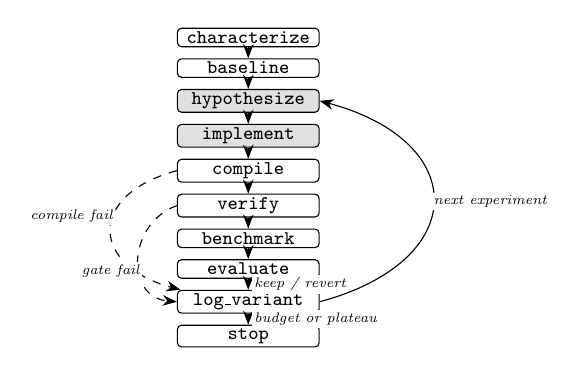
\begin{tikzpicture}[
  >={Stealth[length=1.8mm]},
  state/.style={draw, rounded corners=1.5pt, font=\scriptsize\ttfamily,
    inner xsep=3pt, inner ysep=1.2pt, minimum width=18mm},
  agent/.style={state, fill=black!12},
  glab/.style={font=\tiny\itshape, inner sep=1pt, fill=white},
  node distance=1.4mm]
\node[state] (ch) {characterize};
\node[state, below=of ch] (ba) {baseline};
\node[agent, below=of ba] (hy) {hypothesize};
\node[agent, below=of hy] (im) {implement};
\node[state, below=of im] (co) {compile};
\node[state, below=of co] (ve) {verify};
\node[state, below=of ve] (be) {benchmark};
\node[state, below=of be] (ev) {evaluate};
\node[state, below=of ev] (lv) {log\_variant};
\node[state, below=of lv] (st) {stop};
\foreach \a/\b in {ch/ba, ba/hy, hy/im, im/co, co/ve, ve/be, be/ev}
  \draw[->] (\a) -- (\b);
\draw[->] (ev) -- node[glab, right=1pt] {keep / revert} (lv);
\draw[->] (lv) -- node[glab, right=1pt] {budget or plateau} (st);
\draw[->] (lv.east) to[out=15, in=-15, looseness=2.0]
  node[glab, right=-1pt] {next experiment} (hy.east);
\draw[->, dashed] (co.west) to[out=195, in=165, looseness=2.0]
  node[glab, left=-1pt, pos=0.4] {compile fail} (lv.170);
\draw[->, dashed] (ve.west) to[out=200, in=175, looseness=1.4]
  node[glab, left=-1pt, pos=0.6] {gate fail} (lv.180);
\end{tikzpicture}
\caption{The Seppa loop. Shaded states are the agent's; dashed guard
edges route compile and gate failures to \texttt{log\_variant}, so
\texttt{benchmark} requires a green \texttt{verify}.}
\label{fig:fsm}
\end{figure}


Fig.~\ref{fig:fsm} shows the graph, with two guard edges
to \texttt{log\_variant}, on compile failure and on gate failure, and a
third edge returning \texttt{implement} to \texttt{hypothesize} when the
model submits nothing usable. The guards are ordinary code, from
\texttt{v3d\_flood2\_opt.py}:

\medskip\noindent\begin{minipage}{\linewidth}
\begin{Verbatim}[frame=single,numbers=left,numbersep=3pt,framesep=1.6mm,fontsize=\scriptsize]
("compile_", "verify", expr("compile_ok")),
("compile_", "log_variant", expr("not compile_ok")),
("verify", "benchmark", expr("verify_ok")),
("verify", "log_variant", expr("not verify_ok")),  # guard
("benchmark", "evaluate"),
("evaluate", "log_variant"),
\end{Verbatim}
\end{minipage}\medskip

The benchmark state is reachable only through a green verify. In
operation the Pi runs the server, and any MCP client on the network
drives it through one tool, \texttt{step(action,\ inputs)}, receiving
each state's result and the legal next actions; anything else is
rejected. The server also exposes session utilities
(\texttt{reset\_session}, \texttt{fork\_at}, resource reads) that no
archived session used; Section VIII notes the resampling risk
\texttt{fork\_at} would pose.

The port preserves AutoKernel's loop discipline (audited in
\texttt{docs/autokernel\_fidelity.md}): one focused change per
experiment, a baseline measured first, correctness and timing taken from
the same execution, keep only on a gain of more than 1\%, every
experiment recorded. The port changes who decides. AutoKernel trusts its
agent to run the benchmark and honestly revert failures; in Seppa the
verdict is a deterministic action the model cannot reach. A run ends
after three consecutive non-improvements on gate-passing variants, or at
the budget.

The division of labor was fixed before the sessions ran, and it is worth
stating exactly. The author built the application and the harness, chose
the physics gates, ran the hand-driven sweep of Section V-B, and
supervised sessions. The language model, Claude Sonnet 5 (Anthropic),
driven through the Claude Code client at high reasoning effort, answered
each \texttt{hypothesize} prompt by writing \texttt{implement}'s inputs
(kernel source and host-side parameters) and nothing else. Every
measurement and verdict came from the machine, and no proposed kernel
was edited by hand (transcript in
\texttt{docs/paper/artifacts/claude\_sessions/}). Concretely: the
winning kernel came from the hand-driven sweep and the machine verified
and reproduced it (Section VI); in the one fully agent-driven session
the model tuned only the strip parameter the server already exposed and
never proposed the fused kernel of Section V-B.

For the flood target, \texttt{verify} runs the candidate kernel for 400
steps at 256x256 and applies three checks. Each catches a different way
of being wrong, the standard approach in simulation verification
{[}24{]}, and none requires flood expertise to read. The first is
accuracy: the GPU result must match the same simulation run on the CPU
in double precision, within a normalized mean-square error (NMSE) of
1e-3. The tolerance forgives 32-bit rounding drift but sits six orders
of magnitude above what correct kernels measure, so real bugs land far
outside it. The second is conservation: the simulation adds water only
as rainfall and is built to conserve mass {[}1{]}, so total water on the
grid must stay within 2\% of what rained in; correct kernels drift about
0.003\%. The third is plausibility: water flows downhill, so the deepest
water must end up inside the terrain's basin. A passing gate prints this
in the harness log (here a 4,000-step endurance run; \texttt{verify}
itself runs 400 steps), long lines wrapped:

\medskip\noindent\begin{minipage}{\linewidth}
\begin{Verbatim}[frame=single,numbers=left,numbersep=3pt,framesep=1.6mm,fontsize=\scriptsize]
selected: V3D 7.1.10.2
grid=256^2  steps=4000  time=1.880s  3.07 GFLOP/s
correct(NMSE vs CPU)=yes  NMSE=1.26e-09
mass: rain_injected=5242879.9
  water_total=5242739.3  (conserved vs rain=yes)
pooling: max depth=111.718 at (127,127)
  basin_centre=(128,128)  (pools in basin=yes)
\end{Verbatim}
\end{minipage}\medskip

\section{Case Study: The Flood
Stencil}\label{case-study-the-flood-stencil}

\subsection{The Workload}\label{the-workload}

The simulation runs on a square grid of water depths, and each time step
every cell updates from its four neighbors, the access pattern called a
stencil. The update takes two passes: a flux pass computes how much
water flows across each cell boundary, and a height pass applies those
flows to produce each cell's new depth. The original implementation ran
about 1,045 steps/s at 256x256 (1.51 GFLOP/s), and both shaders compile
without triggering Section II's fallback ladder, which means they never
stress the register allocator. The bottleneck was therefore something
other than register pressure, the demand for more registers than the
hardware has.

\subsection{Falsification Sweep}\label{falsification-sweep}

We treated the bottleneck as something to test, one hypothesis at a
time. Each plausible explanation for the kernel's speed became one
shader variant, and every variant went through the same
compile-verify-benchmark loop that judges the model's proposals. The
ideas themselves are simple. Packing stores two values in one memory
word so the kernel issues fewer loads. Fusion merges the two passes into
a single kernel launch, removing the buffer and the synchronization
barrier between them. Strip-mining gives each GPU thread a short column
of cells instead of one, spreading the fixed cost of starting a thread
over more work. Every variant passed all three gates. Speeds come from
400-step runs at 256x256 on the parameterized \texttt{vkflood2} harness.
Its host loop is faster than the original application's when running
identical kernels, about 1,345 steps/s against 1,045, and mixing the two
would inflate every ratio, so every comparison in this paper is within
\texttt{vkflood2}. Table~\ref{tab:sweep} shows the
sweep. Percentages in the table are relative to its baseline, about
1,345 steps/s (1.94 GFLOP/s); the packed variant's 1.93 is within noise
of it, hence no change.

{\def\LTcaptype{none} % do not increment counter
\begin{table}[!t]\caption{Falsification sweep: 400 steps at 256x256 in the \mbox{vkflood2} harness}\label{tab:sweep}\centering\footnotesize\setlength{\tabcolsep}{2.5pt}\renewcommand{\arraystretch}{1.15}\begin{tabular}{@{}
  >{\raggedright\arraybackslash}p{(\linewidth - 4\tabcolsep) * \real{0.3667}}
  >{\raggedright\arraybackslash}p{(\linewidth - 4\tabcolsep) * \real{0.3000}}
  >{\raggedright\arraybackslash}p{(\linewidth - 4\tabcolsep) * \real{0.3333}}@{}}
\toprule
Variant & Hypothesis tested & Result \\
\midrule
Packed vec2 state (water, surface) halving flux-pass loads & Memory-op
count is the bound & 1.93 GFLOP/s, no change: falsified \\
Fused single-dispatch step (flux buffer eliminated) & Traffic and
barriers are the bound & 2.04 GFLOP/s, +5\%: mostly falsified \\
2 cells per invocation (strip-mined dispatch) & Fixed per-invocation
cost is the bound & 2.40 GFLOP/s, +23\%: supported \\
4 cells per invocation & More strip is better & 2.35 GFLOP/s: falsified,
register pressure \\
Fused + 2 cells per invocation (\texttt{fused2s.comp}) & The wins stack
& 3.08 GFLOP/s, +59\% \\
\bottomrule
\end{tabular}\end{table}
}

The outcome ran against the obvious expectation. Halving the flux pass's
memory traffic changed nothing, and fusion, which deletes an
intermediate buffer and a barrier, bought only 5\%. Fixed per-invocation
cost dominated: each invocation does so little arithmetic that launch
overhead swamps it, and giving each thread two cells beat every
memory-system optimization we tried; four cells gave the gain back to
register pressure. The sweep's own numbers size that cost: strip-2
removes 65,536 invocations per step and saves about 140 microseconds,
near 2 ns per invocation, about two clock cycles, the scale of starting
a thread itself. Two hardware details shaped the final kernel. Strips
run vertically: a subgroup's 16 lanes are horizontal neighbors, so when
each lane walks down its own short column, the subgroup's loads at every
row stay on adjacent addresses. The kernel also consumes each flux value
as it is produced; holding all four alive fails register allocation. The
shipped kernel is 1.58x at 256x256: 1.574 to 1.585 across the five
scored reproductions, 1.571 in the July transcript quoted in Section VI,
and 1.59x hand-timed in the sweep. It is 1.41x at 512x512 and 1.18x at
1024x1024, and it holds all gates over 4,000 steps.

\subsection{Action-Space Limits}\label{action-space-limits}

An early version of the harness let the model edit only the shader
source, and a session run against this stencil under that restriction
found nothing; we nearly concluded the kernel was at its limit. The
restriction itself was the problem: every winning change in
Table~\ref{tab:sweep} lives outside the shader. Packing
changes the buffer layout, fusion removes a host-loop stage, and
strip-mining changes the dispatch shape: all host-program decisions.
Once \texttt{implement} accepted the host parameters as well
(\texttt{\{shader,\ height\_shader,\ strip\}}), the machine verified and
kept the fused strip-2 kernel from its own baseline (Section VI). A
plateau can mean the search space is too small even when the hardware
has headroom. Two other targets ran through the same gated loop, each
behind its own correctness gate. A GEMM (dense matrix multiply) improved
from 7.02 to 13.42 GFLOP/s over two rounds, and a de-unrolled llama.cpp
matrix-vector kernel gained 28\% in end-to-end text-generation speed.
Both are recorded only in the running notes, without the archived logs
that back Section VI.

\section{Machine-Checked Reproduction over
MCP}\label{machine-checked-reproduction-over-mcp}

The Pi runs the Theodosia server; a laptop on the same network runs the
driver script \texttt{drive\_flood2\_mcp.py}, which connects over MCP
and issues the loop's actions in order through the \texttt{step} tool.
All measurement happens on the Pi, and the driver only issues requests.

The state machine measures its own baseline (1,346.8 steps/s on
2026-07-11, gates green), receives the fused strip-2 kernel as
experiment 1, compiles it, gates it, benchmarks 2,116.4 steps/s, and
issues its own verdict, numeric fields rounded here to one decimal:

\medskip\noindent\begin{minipage}{\linewidth}
\begin{Verbatim}[frame=single,numbers=left,numbersep=3pt,framesep=1.6mm,fontsize=\scriptsize]
{"exp": 1, "fused": true, "strip": 2,
 "compile_ok": true, "verify_ok": true,
 "steps_per_sec": 2116.4, "best_sps": 2116.4,
 "verdict": "keep"}
\end{Verbatim}
\end{minipage}\medskip

Then the driver tries to cheat: it submits the same kernel with rainfall
injection doubled in one of the two cell updates, a change that compiles
and breaks conservation. The gate fails it; the driver requests
\texttt{benchmark} anyway, and the server answers (two advisory fields
elided):

\medskip\noindent\begin{minipage}{\linewidth}
\begin{Verbatim}[frame=single,numbers=left,numbersep=3pt,framesep=1.6mm,fontsize=\scriptsize]
{"error": "invalid_transition",
 "requested": "benchmark",
 "valid_next_actions": ["log_variant"],
 "message": "action 'benchmark' is not
   reachable from current state. Valid
   actions now: ['log_variant']."}
\end{Verbatim}
\end{minipage}\medskip

The variant is ledgered as revert with a null \texttt{steps\_per\_sec}.
Gates and timing come from one execution, so the caller still sees the
failing kernel's speed (\texttt{verify} reports it as
\texttt{steps\_per\_sec\_if\_kept}); the green gate controls the ledger,
the verdict, and the kept kernel.

How repeatable is this? \texttt{passk\_flood2.py} runs the two-cycle
reproduction k times from cool starts, each run gated to begin below 55
C, scoring a pass when the baseline gates green inside 1,300 to 1,400
steps/s, the fused kernel is kept at 1.5x or better, and the broken
kernel is refused and nulled. Five of five runs passed on 2026-08-09:
baselines 1,348.6 ± 4.1 steps/s, the kept kernel 2,127.7 in every run
(identical at the timer's resolution), speedups 1.574 to 1.585.

One session was fully agent-driven (2026-08-02, a three-experiment
budget given to the proposer). The server's \texttt{characterize}
payload names fixed per-invocation cost as the bound and exposes the
strip parameter, so the session demonstrates the loop's enforcement
alone. The model worked the exposed knob: strip 4 kept at 1,470.6,
+8.8\%; strip 8 hit the register cliff and was reverted at 921.7; strip
6 probed it and was reverted at 1,298.7. It never reached fusion, and
all of its reported numbers came from the machine.

\section{Concurrent CPU and GPU
Execution}\label{concurrent-cpu-and-gpu-execution}

In deployment the GPU loops the simulation while the CPU computes
shelter routes and decodes (Granite 4.0 1B on llama.cpp with
\texttt{-ngl\ 0}, no layers offloaded to the GPU; 4 threads). Decode,
the token-by-token generation phase, is memory-bound: its speed is set
by how fast model weights stream from memory, and that matters because
the two processors share one LPDDR bus.

The campaign turned up one configuration surprise first. With any Vulkan
device visible, llama.cpp places CPU-resident model weights in memory
set aside for GPU transfers (host-pinned and write-combined) even at
\texttt{-ngl\ 0}, memory that is slow for the CPU reads that dominate
decode. Hiding the device with \texttt{GGML\_VK\_VISIBLE\_DEVICES=99}
takes decode from 9.68 to 11.59 tokens/s, a 20\% gain from an
environment variable (A/B from cool starts, llama-bench, 5 repetitions;
raw logs under \texttt{ab\_vkvisible} in
\texttt{docs/paper/artifacts/}). Every number below uses the
hidden-device configuration, which the application ships.

The benchmark script \texttt{conc\_steady\_bench.sh} (under
\texttt{pi/flood/}) measures each kernel alone (cool starts, finished
before heat accumulates), decode alone, and each kernel looping while
decode runs. Each decode-bearing phase gets a cooldown, then a soak of
eight unreported decode repetitions that bring the chip to working
temperature; kernel-alone phases run straight from the cooldown. The
Pi's firmware defends against heat by lowering clocks, gently past a
soft temperature limit and sharply at a hard throttle, and the logs
record which was active. The soak runs a fixed count instead of waiting
on those flags, and the phases landed in different regimes: the
concurrent phases ran soft-limited 70 to 79\% of the time and peaked at
76.3 C; decode alone reached 73.0 C, limited for 3\%. Each decode phase
defines the measurement window: llama-bench generates 64 tokens per
repetition for 20 repetitions, long enough for 12 to 28 flood
completions, and a flood run counts only if it fits inside the window.

An earlier short-window campaign, preserved in \texttt{conc\_bench2/},
read 711.9 steps/s concurrent with decode at 10.3, against this run's
883.4 and 9.6. Aligning the two campaigns on time since decode began
resolves the difference. Concurrent throughput follows a settling curve:
near 73 C the firmware's soft temperature limit begins capping CPU
clocks, decode slows from 10.2 to 9.6 tokens/s, its per-second memory
traffic thins, and the flood rate climbs. The thermal logs record the
cap engaging in both campaigns. The earlier campaign's window covered
decode's first half-minute, before the cap settled: 711.9 ± 76.1 over
its five completions, against 663.3 ± 34.4 for this run's completions
over the same seconds. The segment's decode rates match as well, 10.32
against 10.21; notebook 02 derives the alignment. The measured window
below sits entirely in the capped regime. Within it the rate still
climbs, from 818.6 steps/s over the first quarter to 919.1 over the
last, so the figure below is a window mean on a rising curve. Results
from the steady-state run of 2026-08-10 are in
Table~\ref{tab:conc} (raw logs under
\texttt{conc\_steady} in \texttt{docs/paper/artifacts/}).

{\def\LTcaptype{none} % do not increment counter
\begin{table}[!t]\caption{Concurrent GPU flood and CPU LLM decode}\label{tab:conc}\centering\footnotesize\setlength{\tabcolsep}{2.5pt}\renewcommand{\arraystretch}{1.15}\begin{tabular}{@{}lll@{}}
\toprule
Condition & GPU flood (steps/s) & CPU decode (t/s) \\
\midrule
Optimized kernel alone & 2,128.0 ± 1.7 (n=3) & \\
Original kernel alone & 1,351.4 ± 0.5 (n=3) & \\
Decode alone, 4 threads (post-soak) & & 11.4 ± 0.0 \\
Concurrent, optimized kernel & 883.4 ± 47.1 (n=28) & 9.6 ± 0.2 \\
Concurrent, original kernel & 401.8 ± 8.3 (n=12) & 9.6 ± 0.2 \\
\bottomrule
\end{tabular}\end{table}
}

Three things follow. Co-processing costs the CPU 16\% of its decode and
buys a continuous 883 steps/s of simulation that a CPU-only deployment
does not have. The interference is lopsided: the CPU keeps 84\% of its
rate while the GPU keeps 42\%, as decode traffic crowds the shared bus.
And contention favors the optimized kernel: 1.58x over the original
alone becomes 2.20x concurrent, at identical decode cost (9.6 t/s under
either kernel). Because the rate is still climbing across the window,
883.4 is a conservative estimate of the late-window rate.

\begin{figure}[!t]
\centering
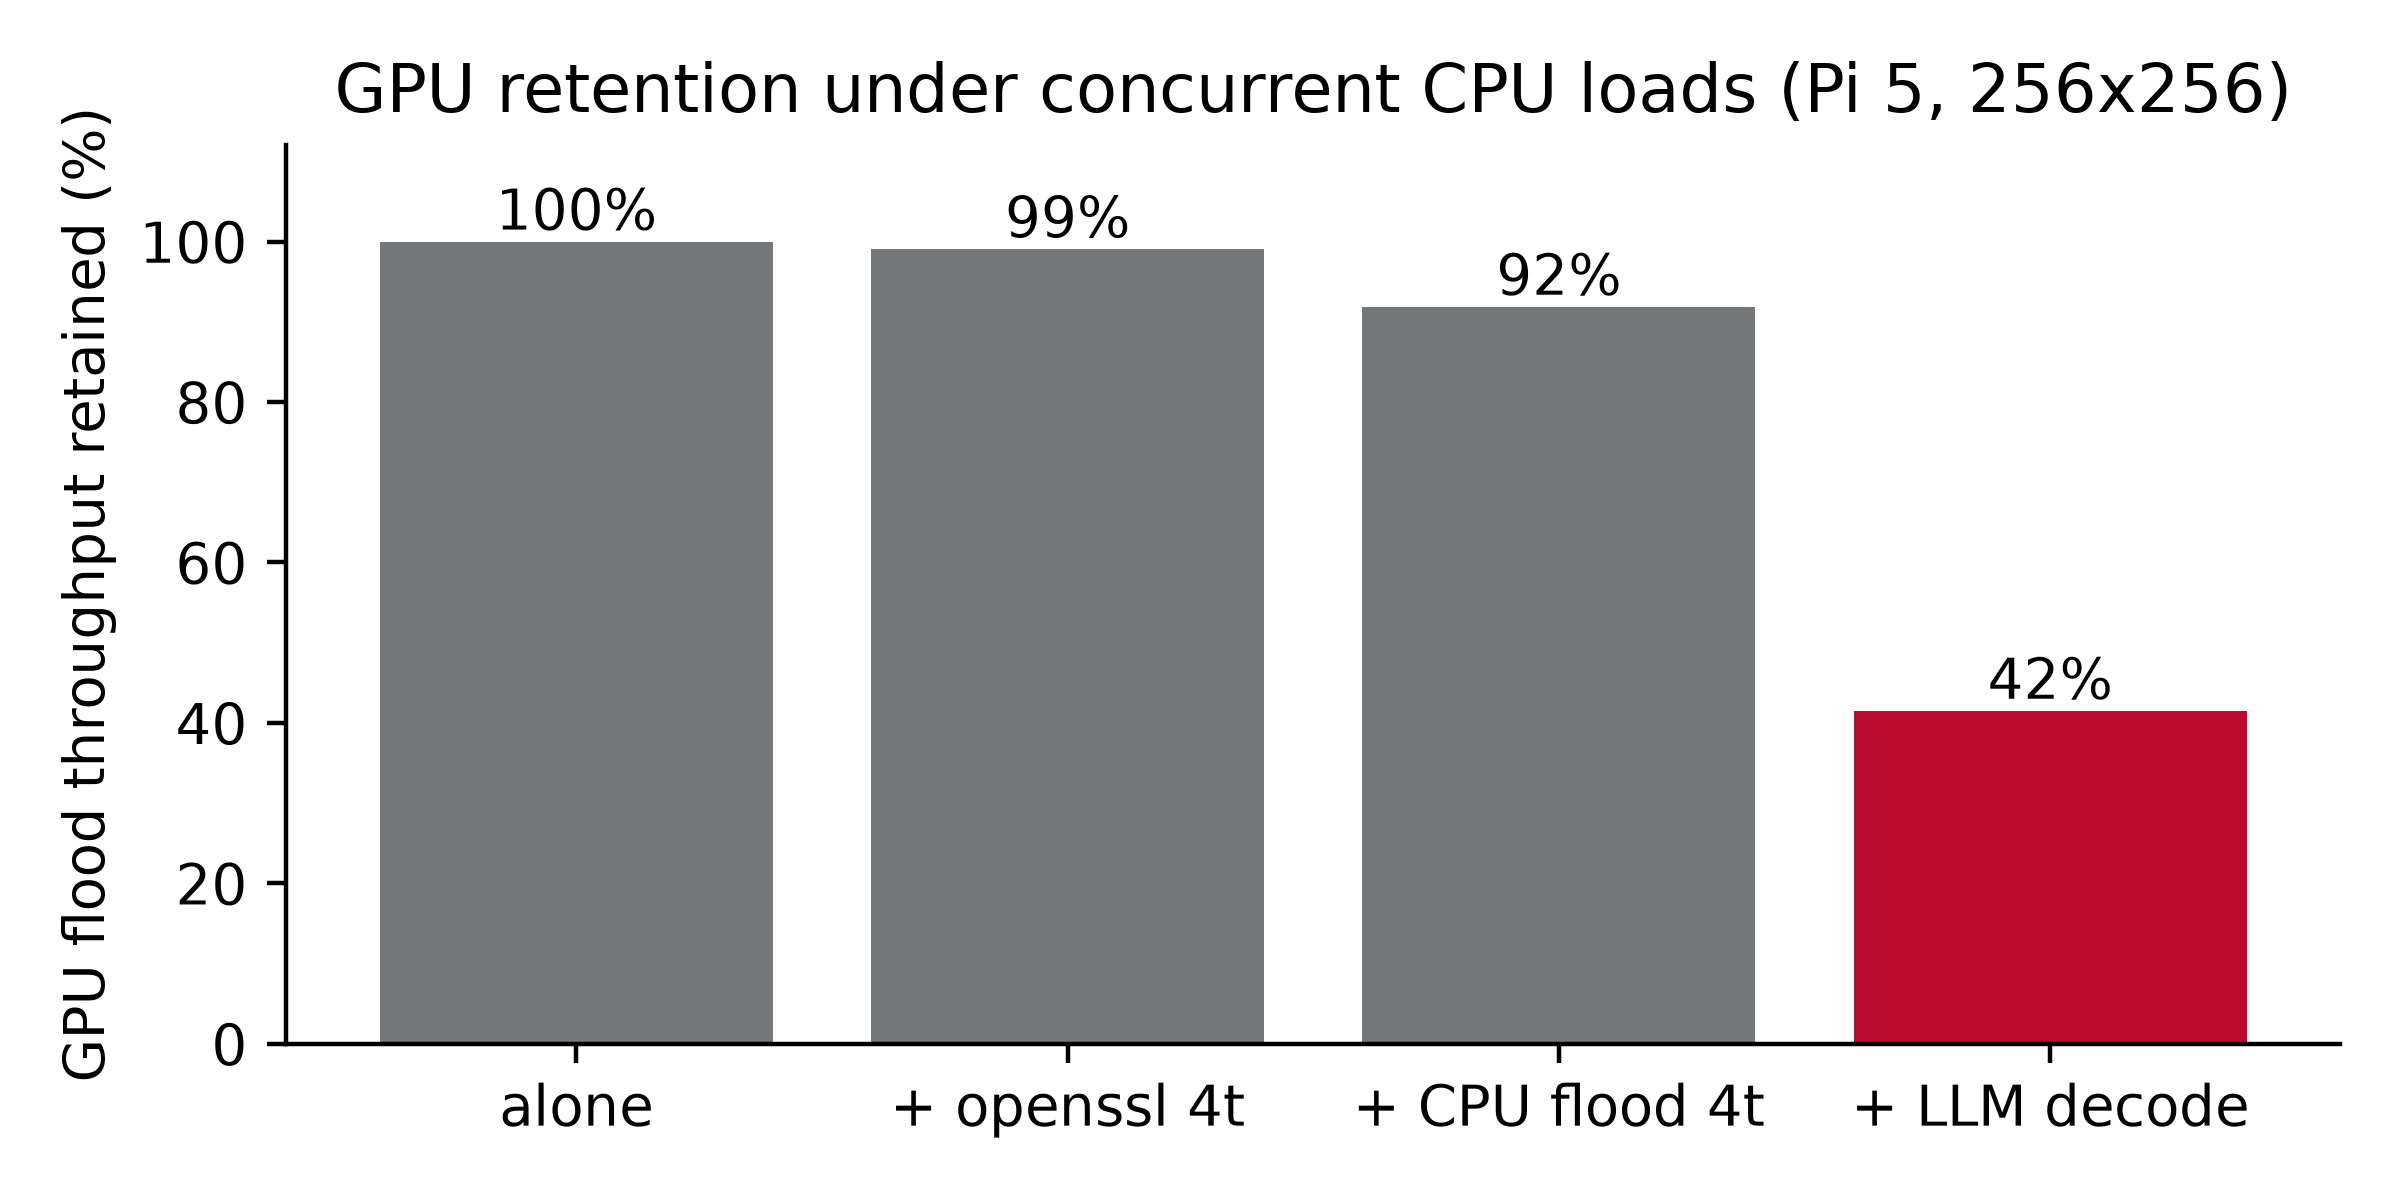
\includegraphics[width=0.92\columnwidth]{gpu_retention.png}
\caption{GPU flood throughput retained beside three concurrent CPU loads, as a percentage of the same kernel running alone. Compute-bound and memory-bound CPU work barely disturb the GPU; language-model decode, which streams weights from DRAM every token, takes it to 42\%. Raw logs under \texttt{genload2} and \texttt{conc\_steady} in \texttt{docs/paper/artifacts/}.}
\label{fig:retention}
\end{figure}

Decode is also the GPU's worst case. Paired with a compute-bound CPU
load (openssl SHA-256, four threads) the GPU keeps 99\% and the load
keeps 88\% of its 16 KB-block throughput; paired with the memory-bound
four-thread CPU flood the GPU keeps 92\% and the load keeps 75\%
(continuous flood-simulation probes over cool-start 60 s windows, both
sides logged under \texttt{genload2} in \texttt{docs/paper/artifacts/}).
These two pairings also bound the thermal confound. Both ran at the same
76.3 C with the soft limit active for 80\% and 70\% of their phases,
against a solo phase that never left 57.6 C, and the GPU still kept 99\%
and 92\%. Clock governance therefore does not explain decode's 42\% on
its own. The GPU is the steadier side of every pairing except decode,
which streams model weights from DRAM every token: interference tracks
the CPU load's memory traffic.

\subsection{The CPU-Only
Counterfactual}\label{the-cpu-only-counterfactual}

Four idle A76 cores run this stencil at 3,852 steps/s, well above the
V3D's 2,128, so the GPU looks unnecessary. The CPU implementation,
\texttt{cpuflood.cpp} in the same directory, is the same update written
with OpenMP, and it passes the same three gates; its error against the
double-precision reference is NMSE 1.46e-11, far inside the 1e-3
tolerance (gate logs in \texttt{cpu\_flood\_bench/}). The companion
script \texttt{cpu\_steady\_bench.sh} measures it alone and sharing the
cores with decode, pinned apart (flood on core 0, decode on 1 to 3) and
oversubscribed (four threads each). The same soak-and-measure protocol
applied; raw logs are under \texttt{cpu\_steady} in
\texttt{docs/paper/artifacts/}. Table~\ref{tab:cpu}
presents the outcome.

{\def\LTcaptype{none} % do not increment counter
\begin{table}[!t]\caption{The CPU-only counterfactual}\label{tab:cpu}\centering\footnotesize\setlength{\tabcolsep}{2.5pt}\renewcommand{\arraystretch}{1.15}\begin{tabular}{@{}
  >{\raggedright\arraybackslash}p{(\linewidth - 4\tabcolsep) * \real{0.4615}}
  >{\raggedright\arraybackslash}p{(\linewidth - 4\tabcolsep) * \real{0.3077}}
  >{\raggedright\arraybackslash}p{(\linewidth - 4\tabcolsep) * \real{0.2308}}@{}}
\toprule
Condition & Flood (steps/s) & CPU decode (t/s) \\
\midrule
CPU flood alone, 1 / 2 / 4 threads & 992.5 / 1,980.5 / 3,852.4 & \\
Decode alone, 3 threads (pinned) & & 11.9 ± 0.0 \\
Partitioned: flood 1t + decode 3t & 678.8 ± 10.6 (n=25) & 8.4 ± 0.1 \\
Oversubscribed: flood 4t + decode 4t & 857.1 ± 181.0 (n=89) & 3.0 ±
0.3 \\
GPU concurrent, optimized (from above) & 883.4 ± 47.1 & 9.6 ± 0.2 \\
\bottomrule
\end{tabular}\end{table}
}

The idle-core number is real but unavailable: in deployment, decode is
always running. Oversubscribed, decode collapses 75\% (llama.cpp's
workers synchronize every token; losing one core stalls all four), and
the flood mean is inflated by bursts between decode repetitions, hence
its ± 181. Partitioned, the best CPU-only arrangement, decode pays a
29\% tax against the GPU split's 16\%; time-slicing (flooding about 23\%
of the time to match 883 steps/s) would cap decode at 8.8 t/s and freeze
guidance during bursts. The GPU split beats the best measured CPU-only
option on both axes, by 30\% on simulation (883.4 ± 47.1 vs 678.8 ±
10.6) and 14\% on decode (9.6 ± 0.2 vs 8.4 ± 0.1): the slower processor
still wins, because the CPU has no spare cycles to sell. The margin is
campaign-dependent, but the direction is not: in the earlier campaign
the decode axis holds and the simulation axis ties within noise (Section
VIII); no measured campaign puts the partitioned scheme ahead on either
axis.

\section{Limitations}\label{limitations}

The measured envelope is one board (Pi 5, V3D 7.1.10.2, Mesa v3dv
25.0.7) and one grid family, and the speedup shrinks as the grid grows.
An operating-system update (kernel 6.12 to 6.18) separates the July and
August campaigns; flood baselines agree across it (1,346.8 before,
1,348.6 ± 4.1 after). The board failed after the August campaign, so
none of these quantities can be re-measured.

The gates are necessary conditions: verification covers one storm
scenario at one grid size. The keep decision rests on a single timing
sample against a 1\% threshold. Across Section VI's five runs the
baseline spread was about 0.3\%, and the kept kernel repeated to the
timer's millisecond resolution, which at 0.188 s is 0.53\% per digit.
The 3,852 steps/s CPU figure assumed a cache-resident 256x256 working
set and may not hold at larger grids.

Section VII carries three asymmetries. The GPU kernel was tuned and the
CPU counterfactual was not; \texttt{cpuflood.cpp} runs the original
two-pass scheme. The thermal operating points were not matched, so clock
governance accounts for part of the 16\% decode cost. And the settled
regime was measured once: the earlier campaign in \texttt{conc\_bench2/}
sampled the pre-cap transient (Section VII aligns the two), so no second
measurement of the settled operating point exists. Taken at face value
the earlier campaign still narrows the simulation margin over the
partitioned scheme to within noise (711.9 ± 76.1 against 678.8 ± 10.6).
The decode margin holds in both campaigns (9.6 and 10.3 against 8.4),
and no measured campaign puts the partitioned scheme ahead on either
axis.

The winning kernel came from the hand-driven sweep, and the agent-driven
session worked a knob the server itself exposed, so the loop's ability
to discover optimizations on its own is untested here. The server's
\texttt{fork\_at} utility rewinds to an earlier state; a caller could
resample a marginal kernel until a draw cleared the 1\% threshold,
\texttt{evaluate} would not notice, and no archived session did so. Full
GPU offload of the language model is blocked by an upstream llama.cpp
Vulkan defect. Numbers without an archived log (the original
application's 1,045 steps/s, the sweep's GFLOP/s column and hand-timed
ratios, the 1.41x and 1.18x at larger grids, and the GEMM and
matrix-vector results) come from the repository's dated running notes.

\section{The Sample Application}\label{the-sample-application}

The sample application {[}7{]} simulates surface flooding over real
terrain {[}1{]}, finds shelter routes by mobility profile {[}2{]}, and
explains the result in plain language, entirely offline; the model never
makes a safety decision, only narrating what the deterministic code
computed. The application lives at \texttt{github.com/msradam/bonbibi}
and was built as an Arm AI Optimization Challenge entry; the harness at
\texttt{github.com/msradam/seppa}. Everything this paper claims was
built for this course, on top of that application. Measurements used its
Granite 4.0 1B configuration. The model file, a 1.63 B-parameter GGUF
(llama.cpp's weight format), appears in llama-bench logs under a
granite-3B size label; the application has since moved to a larger
model. Build commands are in \texttt{pi/flood/README.md}.

\section{Conclusion}\label{conclusion}

Seppa separates proposal from judgment: a language model suggests
kernels for the Raspberry Pi 5's integrated GPU, and a state machine the
model cannot argue with decides what is true about them. On a real flood
stencil this discipline produced a verified 1.58x, proposed in our
hand-driven sweep and reproduced within 1\% by the machine five of five
times, and in the steady-state campaign it holds in deployment: 883
steps/s of simulation beside decode at 84\% of its solo speed. The
evidence in this paper is the gate ledger. The suggestion is open-ended:
commodity edge boards carry more usable silicon than their deployments
exercise, and a loop that cannot misreport its own verdicts is a sound
way to put that silicon to work.

\IEEEtriggeratref{16}
\begin{thebibliography}{24}
\scriptsize
\bibitem{r1} M. Guidolin, A. S. Chen, B. Ghimire, E. C. Keedwell, S.
Djordjević, and D. A. Savić. A weighted cellular automata 2D inundation
model for rapid flood analysis. Environmental Modelling \& Software
84:378-394, 2016.

\bibitem{r2} J. Dibbelt, B. Strasser, and D. Wagner. Customizable Contraction
Hierarchies. ACM Journal of Experimental Algorithmics 21, Article 1.5,
2016.

\bibitem{r3} A. Ouyang, S. Guo, et al.~KernelBench: Can LLMs Write Efficient
GPU Kernels? arXiv:2502.10517, 2025.

\bibitem{r4} X. Li et al.~CUDA-L1: Improving CUDA Optimization via
Contrastive Reinforcement Learning. arXiv:2507.14111; ICLR 2026.

\bibitem{r5} Burr. Apache Software Foundation (incubating).
\url{https://github.com/apache/burr}

\bibitem{r6} Model Context Protocol. \url{https://modelcontextprotocol.io}

\bibitem{r7} Bonbibi: offline flood-aware routing on a Raspberry Pi 5.
\url{https://github.com/msradam/bonbibi}

\bibitem{r8} llama.cpp. ggml-org. \url{https://github.com/ggml-org/llama.cpp}

\bibitem{r9} V3D driver documentation, Mesa 3D.
\url{https://docs.mesa3d.org/drivers/v3d.html}

\bibitem{r10} J. Blocklove, S. Garg, R. Karri, and H. Pearce. Chip-Chat:
Challenges and Opportunities in Conversational Hardware Design. ACM/IEEE
Workshop on Machine Learning for CAD (MLCAD), 2023.

\bibitem{r11} Z. Zhou et al.~Edge Intelligence: Paving the Last Mile of
Artificial Intelligence With Edge Computing. Proc. IEEE 107(8), 2019.

\bibitem{r12} S. Boddu and A. Mukherjee. Efficient Edge Deployment of
Quantized YOLOv4-Tiny for Aerial Emergency Object Detection on Raspberry
Pi 5. arXiv:2506.09300, 2025.

\bibitem{r13} A. Reuther et al.~Survey of Machine Learning Accelerators. IEEE
HPEC, 2020.

\bibitem{r14} The White House. Building Resilient Supply Chains, Revitalizing
American Manufacturing, and Fostering Broad-Based Growth: 100-Day
Reviews under Executive Order 14017. June 2021.

\bibitem{r15} AutoKernel. RightNow AI.
\url{https://github.com/RightNow-AI/autokernel}

\bibitem{r16} Mesa 25.0.7, \texttt{src/broadcom/compiler/vir.c},
\texttt{strategies{[}{]}} compile-fallback table.
\url{https://gitlab.freedesktop.org/mesa/mesa/-/blob/mesa-25.0.7/src/broadcom/compiler/vir.c}

\bibitem{r17} C. Baronio, P. Marsella, B. Pan, et al.~Kevin: Multi-Turn RL
for Generating CUDA Kernels. arXiv:2507.11948, 2025.

\bibitem{r18} J. Woo, S. Zhu, A. Nie, Z. Jia, Y. Wang, and Y. Park. TritonRL:
Training LLMs to Think and Code Triton Without Cheating.
arXiv:2510.17891, 2025.

\bibitem{r19} D. Sarkar. The Correctness Illusion in LLM-Generated GPU
Kernels. arXiv:2606.20128, 2026.

\bibitem{r20} B. Zhao, D. Srikanth, Y. Wu, and Z. Jiang. SpecBench: Measuring
Reward Hacking in Long-Horizon Coding Agents. arXiv:2605.21384, 2026.

\bibitem{r21} B. Romera-Paredes, M. Barekatain, A. Novikov, et
al.~Mathematical discoveries from program search with large language
models. Nature 625:468-475, 2024.

\bibitem{r22} A. Novikov, N. Vu, M. Eisenberger, et al.~AlphaEvolve: A coding
agent for scientific and algorithmic discovery. Google DeepMind, 2025.

\bibitem{r23} S. Thakur, B. Ahmad, H. Pearce, B. Tan, B. Dolan-Gavitt, R.
Karri, and S. Garg. VeriGen: A Large Language Model for Verilog Code
Generation. ACM TODAES, 2024.

\bibitem{r24} W. L. Oberkampf and C. J. Roy. Verification and Validation in
Scientific Computing. Cambridge University Press, 2010.
\end{thebibliography}
\end{document}
